\documentclass{tufte-book}
\title{考研数学一}
\author{肖书奇}
\publisher{2022年}
\usepackage{ifxetex}% For compatibility with xelatex engine
    \ifxetex
    \newcommand{\textls}[2][5]{%
        \begingroup\addfontfeatures{LetterSpace=#1}#2\endgroup
    }
    \renewcommand{\allcapsspacing}[1]{\textls[15]{#1}}
    \renewcommand{\smallcapsspacing}[1]{\textls[10]{#1}}
    \renewcommand{\allcaps}[1]{\textls[15]{\MakeTextUppercase{#1}}}
    \renewcommand{\smallcaps}[1]{\smallcapsspacing{\scshape\MakeTextLowercase{#1}}}
    \renewcommand{\textsc}[1]{\smallcapsspacing{\textsmallcaps{#1}}}
    \usepackage[osf,sc]{mathpazo} % tufte style font
    \usepackage[scaled=0.90]{helvet} % tufte style font
    \usepackage[scaled=0.85]{beramono} % tufte style font
    \fi
\usepackage{ctex} % 支持中文
\usepackage{xeCJK}% 支持中文
    \xeCJKsetup{PunctStyle=kaiming}  % 设置中文标点符号,开明式
    % \xeCJKsetup{PunctStyle=quanjiao} % 设置中文标点符号,全角式
    % \setCJKmainfont{仓耳今楷05-6763}      % 设置正文罗马族的 CJK 字体,影响 \rmfamily 和 \textrm 的字体。
    \setCJKmainfont{STZhongsong}      % 设置正文罗马族的 CJK 字体,影响 \rmfamily 和 \textrm 的字体。
    \setCJKsansfont{STZhongsong}  % 设置正文无衬线族的 CJK 字体,影响 \sffamily 和 \textsf 的字体。
    \setCJKmonofont{SimHei}          % 设置正文等宽族的 CJK 字体,影响 \ttfamily 和 \texttt 的字体。
\usepackage{amsmath} % For AMS math support
\usepackage{amssymb} % For AMS math support
\usepackage{amsfonts} % For AMS math support
\usepackage{booktabs} % For nicely typeset tabular material
\usepackage{makecell} % For multiple lines in one cell in table environment
\usepackage{diagbox}
\usepackage{graphicx} % For graphics / images
    \setkeys{Gin}{width=\linewidth,totalheight=\textheight,keepaspectratio} % Set default scale globally
    \graphicspath{{../graphics/}} % Set paths to search for images
\usepackage{makeidx} % For index
    \makeindex
\usepackage{romannum} % For Roman numbers
\usepackage[dvipsnames]{xcolor} % For various colors
    % \pagecolor{black}
    % \color{white}
\hypersetup{colorlinks} % For colored hyperlinks             
\setcitationfont{\normalfont\footnotesize\color{gray}}
\begin{document}
\frontmatter% Front matter
\maketitle
\tableofcontents% TOC

\chapter*{关于数学学习}
知识的三种属性与其理想载体
\begin{itemize}
    \item 理解性:故事书
    \item 程序性:流程图
    \item 记忆性:工具书
\end{itemize}
\section{如何讲好故事}
\par 定义(结构)是逻辑上的起点,却是学科发展的终点。明确各个定义的逻辑关系,阐明其背景与动机。
\par 定理(性质)分清主次,区分基本性质与重要定理。\sidenote{体系的核心与逻辑脚手架,自然的推论与惊人的发现}
\par 同一个对象,追求不同的理解角度;不同的对象,看出联系。
\marginnote{自然语言与形式语言默写定义和定理,指出关键细节(如限制条件)。定理需要掌握证明思路与使用方法,收集“触发器”。}

\chapter*{待填}
\par 第一章
\begin{itemize}
    \item 区分公理与自然推论
\end{itemize}
\par 第二章
\begin{itemize}
    \item 连通性
\end{itemize}
\par 第三章
\begin{itemize}
    \item 上下极限与根、比值审敛法的应用
    \item 柯西稠密审敛法的应用
    \item 非主干知识
    \item 上下极限性质的证明
\end{itemize}
\par 第四章
\begin{itemize}
    \item 洛必达法则的特例
    \item 所有的不定式
    \item 柯西余项的泰勒定理
    \item 所有的证明
\end{itemize}
% Start the main matter (normal chapters)
\mainmatter

\part{高等数学}

\chapter{实数、复数、Euclidean空间}

\section{实数}
实数的公理化定义\sidenote{戴德金分割提供了具体构造方法}
\sidenote{预备知识:域、有序集、有序域、界、最小上界、最小上界性质}:有序域、最小上界性质
\section{复数}
\par 定义复数及其加法、乘法。定义虚数单位\sidenote{提供了另一种等价的复数刻画,使复数乘法与实数乘法相协调。},定义实部、虚部与共轭。
\section{Euclidean空间}
\par 定义Euclidean向量及其加法、数乘、内积、范数。
\chapter{拓扑基础}
\section{可数集与不可数集}
\begin{marginfigure}
    \centering
    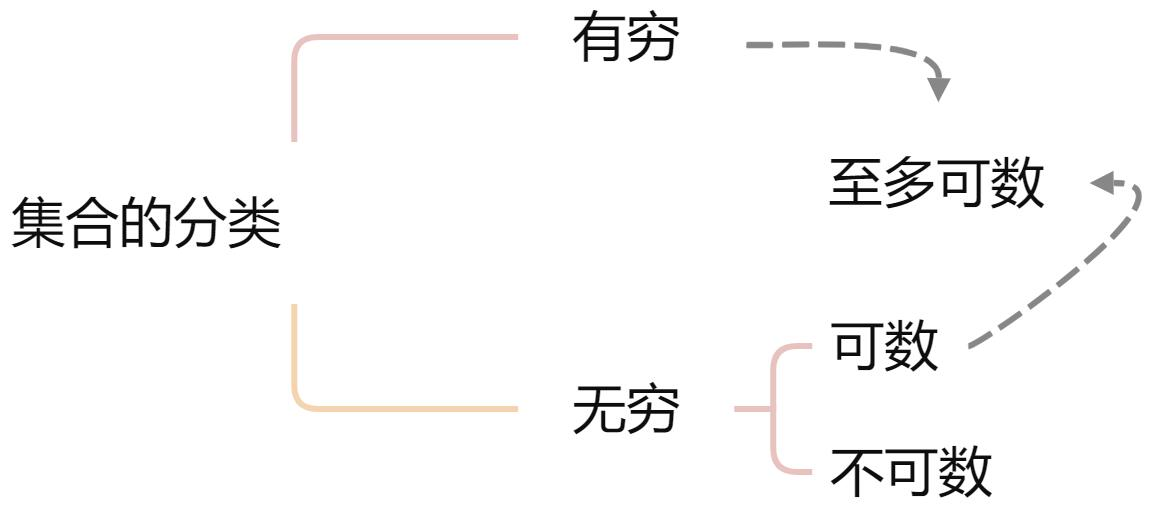
\includegraphics{可数集与不可数集.jpg}
    \caption{集合的分类}
\end{marginfigure}
根据与自然数建立等价映射的可行性,为“无限”分类。
\sidenote{经典命题(Cantor对角线法)
    \begin{itemize}
        \item 可数个可数集的并集可数
        \item 有理数可数
        \item 实数不可数
    \end{itemize}
}
\section{度量空间}
\par 距离函数的公理化定义:半正定性、对称性、次可加性。
\par 点集拓扑的12个基本概念:邻域、内点、聚点、孤立点、开集、闭集、有界集、完美集、稠密集、凸集、紧集、连通集。\sidenote{
    关于邻域、内点、聚点、开集、闭集的基本性质
    \begin{itemize}
        \item 邻域是开集
        \item 某集合的聚点的任意邻域包含该集合的无穷元素
        \item 有穷集合不可能有聚点
        \item 某集合是开(闭)集等价于其补集为(开)集
        \item 任意个开集的并集是开集;任意个闭集的交集是闭集;任意有限个开集的交集是开集;任意有限个闭集的并集是闭集
        \item 集合的封闭是包含它的最小闭集;集合是闭集等价于与自身的封闭相等
        \item 集合的开/闭具有相对性;集合是相对开集(相对度量空间的某个子集是开集)等价于其等于某个绝对开集(相对整个度量空间的开集)与背景集合的交集
        \item 实数上的有界集若是闭集,则其确界在集合内部
    \end{itemize}
}
\section{紧集}
\par 利用开覆盖定义紧集。
\sidenote{关于紧集的基本性质
    \begin{itemize}
        \item 紧性与嵌入的背景集合无关(绝对紧性等价于相对紧性)
        \item 紧集是闭集
        \item 紧集的闭子集是紧集
        \item 任意紧集簇中的任意有限紧集的交集非空,则该紧集簇的交集非空;单调缩小的非空紧集序列的交集非空;
        \item 实数域的闭区间是紧集;Euclidean空间的k-cell是紧集(Bolzano二分区间法)
    \end{itemize}
}
核心是实数/复数/Euclidean空间两个常用的紧性定理,Borel-Heine定理和Weierstrass定理。
% \par Borel-Heine定理:\(E\subset \mathrm{R}^k\),以下命题等价
% \begin{itemize}
%     \item \(E\)是紧集
%     \item \(E\)是有界闭集
%     \item 任何\(E\)的无穷子集都有聚点,且该聚点在\(E\)中
% \end{itemize}
% \par Weierstrass定理:\(\mathrm{R}^k\)的任意有界无穷子集都存在聚点。

\chapter{序列与级数}
\section{序列}
定义收敛序列\sidenote{
    收敛序列的基本性质
    \begin{itemize}
        \item 极限唯一
        \item 收敛序列有界
        \item \(\{p_n\}\)收敛于\(p\)等价于\(p\)的任意邻域包含除了\(\{p_n\}\)有限个点以外的所有点
        \item \(E\subset X\)有聚点\(p\),必存在\(\{p_n\}\subset E\)以\(p\)为极限
    \end{itemize}
},重要结论是在实数、复数、Euclidean空间上的收敛序列的极限运算与算术运算的关系。
% \(X\)是度量空间,\(\{p_n\}\subset X\),\(p\in X\)
% \[\lim_{n\to\infty}p_n=p:=\forall \epsilon>0\;\exists N\in\mathbb{N}\;\forall n>N\left(n>N\Rightarrow \operatorname{d}_X(p_n,p) < \epsilon\right)\]
\par 定义子列\sidenote{子列的基本性质
    \begin{itemize}
        \item 序列的全部收敛子列的极限构成的集合是闭集
    \end{itemize}
},重要结论是任意有界序列必存在收敛子列。(Bolzano-Weierstrass致密性定理)
\par 定义Cauchy列\sidenote{
    Cauchy列的基本性质
    \begin{itemize}
        \item 收敛序列必是柯西列
    \end{itemize}
},重要结论是实数、复数、Euclidean空间的柯西列必然收敛\sidenote{本质是紧度量空间上的柯西列必收敛}。定义完备性。
\par 定义实数序列的单调性,重要结论是单调且有界的序列必然收敛。
\par 定义实数序列的上、下极限。\sidenote{上、下极限的基本性质\par\(E:=\{\text{全部收敛子列的极限值}\}\)
    \begin{itemize}
        \item \(s^\ast \in E,\; s_\ast \in E\)
        \item \(\begin{aligned}
                  \forall x>s^\ast\Rightarrow \left(\exists N\in \mathbb{N}\; \forall n>N\; (x>s_n)\right) \\
                  \forall x<s_\ast\Rightarrow \left(\exists N\in \mathbb{N}\; \forall n>N\; (x<s_n)\right) \\
              \end{aligned}\)
        \item \(\left(\exists N\in\mathbb{N}\;\forall n>N\; (s_n\geq t_n)\right) \Rightarrow \left(s^\ast \geq t^\ast\;\wedge\; s_\ast \geq t_\ast\right) \)
    \end{itemize}
}
\par 经典实序列极限如下:
\begin{table}
    \centering
    \begin{tabular}{ccc}
        \toprule
        参数                                 & 收敛序列                                                     & 极限  \\
        \midrule
        \(p>0\)                              & \(\displaystyle \lim_{n\to\infty}\dfrac{1}{n^p}\)            & \(0\) \\
        \midrule
        \(p>0\)                              & \(\displaystyle \lim_{n\to\infty}\sqrt[n]{p}\)               & \(1\) \\
        \midrule
        \(p>0\;\wedge\;\alpha\in\mathbb{R}\) & \(\displaystyle \lim_{n\to\infty}\dfrac{n^\alpha}{(1+p)^n}\) & \(0\) \\
        \midrule
        \(\vert x\vert<1\)                   & \(\displaystyle \lim_{n\to\infty}x^n\)                       & \(0\) \\
        \midrule
        \diagbox{}{}                         & \(\displaystyle \lim_{n\to\infty}\sqrt[n]{n}\)               & \(1\) \\
        \bottomrule
    \end{tabular}
\end{table}
\section{级数}
\par 在实、复数中定义部分和序列,定义数项级数\sidenote[][-4cm]{
    数项级数的基本性质
    \begin{itemize}
        \item 收敛的数项级数的通项收敛且极限为零
        \item 通项为非负数的实数项级数的收敛性等价于有界性
    \end{itemize}
},重要结论是基于柯西收敛准则刻画级数敛散性的等价条件。
\par 数项级数的敛散判定是重点。比较审敛法\sidenote[][-3.5cm]{比较审敛法
    \begin{itemize}
        \item 敛:除了有限项,通项的绝对值小于等于某收敛级数的通项
        \item 散:除了有限项,通项大于等于某发散级数的通项的绝对值
    \end{itemize}
}、柯西稠密审敛法\sidenote[][-1.5cm]{柯西稠密审敛法:
若通项\(a_n\)是单调\textcolor{BrickRed}{递减}的\textcolor{BrickRed}{非负}数列,则\(\sum a_n\)与\(\sum 2^ka_{2^k}\)敛散性相同。
}、根审敛法\sidenote[][-1cm]{根审敛法:
    \(\displaystyle\alpha:=\operatornamewithlimits{lim\;sup}_{n\to\infty}\sqrt[n]{\vert a_n\vert}\)
    \begin{itemize}
        \item \(\alpha < 1\),\(\sum a_n\)收敛
        \item \(\alpha > 1\),\(\sum a_n\)发散
        \item \(\alpha = 1\),\(\sum a_n\)敛散性未知
    \end{itemize}
}、比值审敛法\sidenote[][]{比值审敛法:
    \begin{itemize}
        \item 若\(\displaystyle\operatornamewithlimits{\lim\;\sup}_{n\to\infty}\vert\dfrac{a_{n+1}}{a_n}\vert<1\),则\(\sum a_n\)收敛
        \item 若\(\exists N\in\mathbb{N}\; \forall n>N\;\left(\left\vert\dfrac{a_{n+1}}{a_{n}}\geq 1\right\vert\right)\),则\(\sum a_n\)发散
    \end{itemize}
    另外,若根审敛法无法判断,则比值审敛法同样无效。
}
\par 经典数项级数如下(比较审敛法和柯西稠密判定法可判定):
\begin{table}
    \centering
    \begin{tabular}{ccc}
        \toprule
        参数            & 级数                                                   & 敛散性 \\
        \midrule
        \(0\leq x < 1\) & \(\displaystyle \sum x^n = \frac{1}{1-x}\)             & 收敛   \\
        \midrule
        \(x\geq 1\)     & \(\displaystyle \sum x^n \)                            & 发散   \\
        \midrule
        \(p\leq 1\)     & \(\displaystyle \sum\frac{1}{n^p}\)                    & 发散   \\
        \midrule
        \(p>1\)         & \(\displaystyle \sum\frac{1}{n^p}\)                    & 收敛   \\
        \midrule
        \(p\leq 1\)     & \(\displaystyle \sum\frac{1}{n(\log n)^p}\)            & 发散   \\
        \midrule
        \(p>1\)         & \(\displaystyle \sum\frac{1}{n(\log n)^p}\)            & 收敛   \\
        \midrule
        \diagbox{}{}    & \(\displaystyle \sum\frac{1}{n\log n\log \log n}\)     & 发散   \\
        \midrule
        \diagbox{}{}    & \(\displaystyle \sum\frac{1}{n\log n(\log \log n)^2}\) & 收敛   \\
        \bottomrule
    \end{tabular}
\end{table}
\par 定义函数项级数,定义幂级数(实/复数域)。重要结论是幂级数收敛域是圆形,及其收敛半径的表达式。\sidenote{\(R:=\dfrac{1}{\operatornamewithlimits{lim\;sup}_{n\to\infty}\sqrt[n]{\vert c_n \vert}}\)}
\par 定义级数的绝对收敛。重要结论是级数绝对收敛是收敛的充分非必要条件。

\chapter{连续}
\par 定义映射在某点处的极限。重要结论是沟通了序列极限与映射极限的Heine定理\sidenote{
    映射极限的基本性质
    \begin{itemize}
        \item 映射在某点若存在极限则极限唯一
    \end{itemize}
},以及实数、复数、Euclidean空间函数极限运算与算术运算的关系。
\par 定义映射在某点处的连续性。重要定理是连续性与极限的关系\sidenote{特例:孤立点};连续映射的复合仍连续;实、复数、Euclidean空间里的各种基本运算(加、减、乘、除、向量加法、数乘、内积、直积、限定)保持映射的连续性。
\par 连续映射具有丰富的拓扑性质,可以利用开、闭集作连续性的等价刻画。重要定理是连续映射与紧集、连通集的关系:连续映射将紧集映射为紧集(有界性定理、最值定理),将连通集映射为连通集(介值定理)。
\par 定义一致连续,显然一致连续蕴含连续,重要定理是紧集上的连续与一致连续等价。
\par 对于以实数为自变量的函数,可以定义左极限与右极限,从而为不连续点分类。重要定理是关于单调函数的不连续性。
\par 定义实、复数、Euclidean空间的扩充与广义邻域,定义广义极限(无穷处的极限)与无穷极限(极限值是无穷)。重新考察了极限(包含广义与无穷)与基本运算的关系,从而为无穷定义了几种运算,悬而未决的不定式是重点\sidenote{常见不定式
    \begin{itemize}
        \item \(\dfrac{\infty}{\infty}\)
        \item \(\dfrac{0}{0}\)
    \end{itemize}
}。

\chapter{导数}

定义实函数\sidenote{自、因变量皆为实数}的导数与单侧导数\sidenote{
    理解导数的两种方式:
    \begin{itemize}
        \item 瞬时变化率(Newton)
        \item 最佳的局部线性近似(Leibniz)
    \end{itemize}
}
\sidenote{导数的基本性质
    \begin{itemize}
        \item 若可导,导数唯一
        \item 可导蕴含连续
    \end{itemize}
}。重要定理是求导运算与算术运算的关系;复合函数的求导链式法则。
\par 定义极小、极大值。重要定理是若极值点可导\sidenote{极值点处可能不可导},则导数为零。
\par 三大微分中值定理\sidenote{微分中值定理的前提条件
\begin{itemize}
    \item 闭区间连续\(f,g\in C^0[a,b]\)
    \item 开区间可导\(\forall x\in(a,b)\;\exists\;f'(x),g'(x)\)
\end{itemize}
Rolle中值定理
\[f(a)=f(b)\Rightarrow \left(\exists \xi\in[a,b] \; f'(\xi)=0\right)\]
Lagrange中值定理
\[\exists \xi\in(a,b) \; f(\xi)=\frac{f(b)-f(a)}{b-a}\]
Cauchy中值定理
\[\exists \xi\in(a,b) \; ((f(a)-f(b))g'(\xi) = (g(a)-g(b))f'(\xi)\]
},掌握其应用。
\par 导数未必连续,但必有介值性。
\par 定义高阶导数。
\par L'Hospital's法则提供了某种不定式极限的考察方法,注意其应用条件。\sidenote{L'Hospital's法则
    \begin{itemize}
        \item \(a\in\overline{\mathrm{R}}\),\(f(x)\)和\(g(x)\)都在\(a\)点的单侧开邻域可导
        \item \(\lim_{x\to a}\dfrac{f^\prime(x)}{g^\prime(x)}\)存在
    \end{itemize}
    并且满足以下其一
    \begin{enumerate}
        \item \(x\to a\), \(f(x)\to\infty\;\wedge\;g(x)\to\infty\)
        \item \(x\to a\), \(f(x)\to0\;\wedge\;g(x)\to 0\)
    \end{enumerate}
    则\[\lim_{x\to a}\dfrac{f(x)}{g(x)}=\lim_{x\to a}\dfrac{f^\prime(x)}{g^\prime(x)}\]
}
\par Taylor's定理阐明了最佳的局部多项式近似与各阶导数的关系。\sidenote{
    \(f\in C^n\)
    \[f(x) = f(a) + \sum^{n}_{k=1}\frac{f^{(k)}(x)}{k!}(x-a)^k + o\left((x-a)^n\right)\]
}

\chapter{Riemann-Stieltjes积分}

积分两要素:被积对象与积分区域。Riemann-Stieltjes积分是实函数在闭区间上的积分。\par 利用分割、Darboux上/下和、Darboux上/下积分,定义R-S积分\sidenote{
    Darboux定义的基本性质
    \begin{itemize}
        \item 若分割更加精细,则达布上和会更小,达布下和会更大(也可以不变)
        \item 达布下积分小于等于达布上积分
        \item R-S可积等价于存在分割使达布上下和任意地接近
        \item R-S可积等价于“达布任意和”与积分值可以任意地接近(定积分求的是面积的精确值,只要你承认长方形的面积等于长乘以高)
    \end{itemize}
}。众多可积性定理给出了R-S可积的充分条件\sidenote{
    R-S可积性定理
    \begin{itemize}
        \item 闭区间上的连续函数可积
        \item 闭区间上的单调函数可积(\(\alpha\)连续)
        \item 闭区间上的有界且间断点可数的函数可积(\(\alpha\)在被积函数的间断点处连续)
        \item 可积函数的复合函数仍可积
        \item 可积函数的加、减、乘、除仍可积
    \end{itemize}
}。
\par 易证R-S积分的基本性质\sidenote{
    R-S积分的基本性质
    \begin{itemize}
        \item 双线性
        \item 区间可加性
        \item 抽样性质(\(\alpha:=\)单位阶跃函数,等价于与Dirac函数卷积)
    \end{itemize}
}。\par 几个经典的\(\alpha\)构造展示了R-S积分相对Riemann积分的优越之处——利用单位阶跃函数将积分值转化为级数极限
,利用\(\alpha\)的导数将R-S积分转化为Riemann积分(重要),利用\(\alpha\)的复合可完整地说明积分的换元公式(重要)。\sidenote{R-S积分的很多限制条件,工科生可能永远不会遇到。目前理论有限,对于各种条件的说明也不够精确。}
\par 定义变上限积分\sidenote{
    首先,变上限积分是一个函数,是借助R-S可积函数自然构造出来的一个函数。它的性质很好:在整个闭区间上连续;若被积函数在某处连续,则它在该处可导。
}以后,微积分基本定理呼之欲出。
\par 分部积分公式对应的是乘法的导数运算。
% \section{序列的极限}

% \subsection{定义}

% \[ \{p_n\} \subset X \]
% \[\lim_{n\to \infty} p_n = p := \forall \epsilon>0\;\exists N\in\mathbb{N}\;\forall n>N\;(\operatorname{d}_X(p_n,p) < \epsilon)\]

% % \[\lim_{n\to \infty} p_n = p := \forall \epsilon>0 \exists N\in\mathbb{N} \forall n>N (\vert p_n-p \vert < \epsilon)\]

% \marginnote{
%     利用定义证明极限时常用的三角不等式
%     \[
%         \begin{aligned}
%             \vert a \vert + \vert b \vert \geq \vert a + b \vert \\
%             \vert a \vert + \vert b \vert \geq \vert a - b \vert \\
%             \vert a \vert - \vert b \vert \leq \vert a + b \vert \\
%             \vert a \vert - \vert b \vert \leq \vert a - b \vert \\
%         \end{aligned}
%     \]
% }

% \subsection{性质}

% \begin{table}
%     \centering
%     \begin{tabular}{cccc}
%         \toprule
%                  & 内容                  & 应用 & 证明 \\
%         \midrule
%         通用性质 & \makecell{有限值/聚点               \\唯一性\\有界性\\有限项可去} &  &    \\
%         算术运算 & 传递性                &      &      \\
%         不等式   & 传递性                &      &      \\
%         \bottomrule
%     \end{tabular}
% \end{table}

% \subsection{判定}

% \begin{table}[htbp]
%     \centering
%     \begin{tabular}{cccc}
%         \toprule
%                      & 内容                         & 应用 & 证明 \\
%         \midrule
%         柯西收敛定理 & 柯西列与收敛性等价           &      &      \\
%         单调收敛定理 & 对于单调序列,收敛等价于有界 &             \\
%         \bottomrule
%     \end{tabular}
% \end{table}

% \subsection{例子}

% \[\lim_{n\to\infty}\frac{n}{q^n}=0 \quad(q>1)\]
% \[\lim_{n\to\infty}\sqrt[n]{n}=1\]
% \[\lim_{n\to\infty}\sqrt[n]{a}=1 \quad (a>0)\]
% \[\lim_{n\to\infty}\frac{q^n}{n!}=0 \quad(q\in\mathbb{R})\]



\part{线性代数}

\chapter{线性映射}
\section{线性映射的概念}
\section{线性映射构成的线性空间}
\section{有限维线性映射的基本定理}
\section{线性映射的矩阵}
\section{线性变换与其逆的概念}
\section{积空间与商空间}
\section{对偶与秩}
\par 在线性代数中,我们接触的第一个对偶关系是向量和线性泛函的对偶。\sidenote{类似“点动成线,线动成点”。}
顺理成章,有
\begin{itemize}
    \item 线性空间的对偶(对偶空间)属于线性泛函空间;
    \item 线性空间的基的对偶(对偶基)属于线性泛函空间的基;
    \item 线性空间之间的映射的对偶(对偶映射)属于线性泛函空间之间的映射。
\end{itemize}
\par 严格定义如下:\sidenote{需额外证明对偶基是基。重点关注对偶映射的构造方式。}
\[V^\prime := \mathcal{L}(V,\mathbb{F})\]
\[\{v_k\}=: \text{A basis of } V,\quad \varphi_k(v_j):=\begin{cases}1&j=k\\0&j\neq k\end{cases}\]
\[T:V\mapsto W,\quad T^\prime(\varphi) := \varphi \circ T \in \mathcal{L}(W^\prime,V^\prime)\]
\par 根据定义,可得一些基本性质,见表格\ref{线性代数的对偶基本性质}。
\begin{margintable}
    \centering
    \begin{tabular}{cc}
        \toprule
        命名           & 内容                                \\
        \midrule
        对偶同构律     & \(\dim V' = V\)                     \\
        对偶映射运算律 & \makecell{\(ST=T^\prime S^\prime \) \\ \((\lambda T)^\prime=\lambda T^\prime \)\\ \( (S+T)^\prime = S^\prime + T^\prime \)} \\
        \bottomrule
    \end{tabular}
    \caption{线性代数的对偶基本性质}
    \label{线性代数的对偶基本性质}
\end{margintable}
\par 随后利用零化子空间\sidenote{annihilator}研究对偶映射的核与值域。定义为:\sidenote{可以为普通的子集\(U\)定义零化子空间,未必是子空间;定义没有揭示零化子空间是子空间,需额外证明。}
\[U\subset V,\quad U^0_V:=\{\varphi\in V^\prime : \forall u\in U(\varphi(u)=0)\}\]
\par 脚手架:子空间与其零化子空间的维度之和是母空间维度。\sidenote{证明思路:关键在于零化子空间可视作对偶映射的零空间,即\(\forall T\in\mathcal{L}(U, V)\;(\operatorname{null} T^\prime=U^0)\),再取特例\(T(u)=u\),易得\(\dim\operatorname{range} T^\prime = \dim U\),再应用秩零定理得证。}
\[\dim V = \dim U + \dim U^0\]
\par 应用秩零定理,可以得到结论,见表格\ref{对偶映射的性质}。\sidenote{原映射与对偶映射的核与值域的关系对于无限维线性代数仍旧成立。(无需秩零定理即可证明)}
\begin{table}
    \centering
    \begin{tabular}{cc}
        \toprule
        命名           & 内容                                                                           \\
        \midrule
        核与值域的对偶 & \makecell{\(\operatorname{null}T^\prime = (\operatorname{range}T)^0\)          \\ \(\operatorname{range}T^\prime = (\operatorname{null}T)^0\)}\\
        单与满的对偶   & \makecell{\(T^\prime\) is surjective \(\Leftrightarrow\) \(T\) is injective    \\ \(T^\prime\) is injective \(\Leftrightarrow\) \(T\) is surjective} \\
        维度关系       & \makecell{\(\dim \operatorname{range} T^\prime = \dim \operatorname{range} T\) \\ \(\dim\operatorname{null} T^\prime = \dim\operatorname{null} T + \dim W - \dim V\) } \\
        \bottomrule
    \end{tabular}
    \caption{对偶映射的性质}
    \label{对偶映射的性质}
\end{table}
\par 最后研究对偶映射的矩阵。结论是矩阵的转置与线性映射的对偶等价。自然,对偶映射运算律对应转置矩阵运算律。
\par 在这里适合给出矩阵的秩的概念,先定义行秩与列秩,\sidenote{行向量属于\(\mathbb{F}^{1, n}\),列向量属于\(\mathbb{F}^{m, 1}\)}
\[\operatorname{column\ rank} A := \dim \operatorname{span} \{\text{column vectors of A}\}\]
\[\operatorname{rank\ rank} A := \dim \operatorname{span} \{\text{rank vectors of A}\}\]
显然矩阵的列秩等于对应线性变换的值域的维度。再根据\(\dim \operatorname{range} T = \dim \operatorname{range} T^\prime \),直接推出行秩等于列秩。

\chapter{特征值、特征向量与不变子空间}
本章研究线性变换。\sidenote{线性变换的物理背景较为丰富。线性“变换”的一个特别之处:可以定义其幂运算,构造多项式。值得一提的性质是:\(p(T)q(T)=q(T)p(T)\)}由于线性变换只涉及一个线性空间,很自然的想法就是对这个空间作直和分解,分别考察线性变换的作用效果。\sidenote{线性代数是关于表示的学问,直和表示空间和基的线性组合表示向量的思想是共通的。}
但是,该线性变换对于各个子空间而言,未必是线性变换,可能是线性映射。首先,仅考虑不变子空间的情况——如果某个子空间包含了该线性变换在其上的值域,我们称之为不变子空间。
\[T\in\mathcal{L}(V),\quad \text{a subspace } U\text{ is invariant}:= (u\in U \Rightarrow Tu\in U)\]
\par 显然,对于任何线性变换,其零空间和值域都是不变子空间,这是平凡的例子。我们接着考虑最简单也最理想的不变子空间(一维)\sidenote{直和分解的理想结果就是一维子空间}。根据线性空间与线性映射的定义,只能有这种情况:
\(\forall v\in V\;\exists\lambda\in\mathbb{F}\;Tv=\lambda v\)。特征值和特征向量的概念出现了。\sidenote{“只能有这种情况”,所以“存在”即可,但是这个存在显然不能是零向量。}
\[
    \begin{aligned}
         & \lambda \in \mathbb{F}\wedge (\exists v\in V( v\neq 0 \wedge Tv=\lambda v)) \\
         & := \lambda \text{ is an eigen value of }T
    \end{aligned}
\]
\[
    \begin{aligned}
         & \lambda \text{ is an eigen value of }T \wedge v \in V \wedge v \neq 0 \wedge Tv=\lambda v \\
         & := v \text{ is an eigen vector of }T \text{ corresponding to }\lambda
    \end{aligned}
\]
\par 根据定义,可以得到关于特征值与特征向量的几个等价条件。
\sidenote{
    以下命题等价:
    \begin{itemize}
        \item \(\lambda\)是\(T\)的一个特征值;
        \item \(T-\lambda I\)不是单射;
        \item \(T-\lambda I\)不是满射;
        \item \(T-\lambda I\)不可逆;
    \end{itemize}
    以下命题等价:
    \begin{itemize}
        \item \(v\)是\(T\)关于特征值\(\lambda\)的特征向量;
        \item \(v\in\operatorname{null}(T-\lambda I) \wedge v \neq 0\)
    \end{itemize}
}
可以发现\(T-\lambda I\),这个线性变换是非常重要的脚手架,定义特征子空间:
\[E(\lambda,T) := \operatorname{null}(T-\lambda I)\]
也容易证明特征值和特征向量的一些基本性质。\sidenote{
    \begin{itemize}
        \item 不同特征值对应的特征向量必然线性无关(不同特征值对应的特征子空间之和是直和);
        \item 不同特征值的个数至多是维度数目(不同特征值对应的特征子空间之和的维度小于等于母空间维度)。
    \end{itemize}
}
\par 可以利用线性变换的不变子空间诱导出两种变换——限制变换和商变换。\sidenote{根据定义有\(T\vert_U \in \mathcal L(U), T/U\in\mathcal L(V/U)\)。好好体会这种映射是线性、是变换。}暂时没派上用场,先放这儿。
\[T\vert_U(u) := Tu\]
\[(T/U)(v+U):=Tv+U\]
\par 首先应关心存在性问题:不变子空间/特征值/特征向量广泛存在于各种线性空间和线性变换吗?一个重要结论是:\textcolor{BrickRed}{任何非零}\textcolor{BrickRed}{复线性空间上的任何线性变换,必然存在特征值。}\sidenote{“非零”指不是仅有零元素的线性空间。}\sidenote{这说明我们对于不变子空间、特征值、特征向量的研究是有价值的。这个命题的证明方法很多。尽管此时还未引入行列式与特征多项式的概念,但仍可以应用代数基本定理证明此结论。}
\par 下面研究线性变换的矩阵。回忆一下,矩阵表达不仅取决于线性映射本身,还取决于定义空间与到达空间的基的选取。对于线性变换而言,定义空间与到达空间相同,所以选取一组基即可。选基是一门很重要的学问,我们的目标是为线性变换选取一组基,使得对应矩阵的形式最简单。问题来了:什么是最简单?具体怎么选?
\par 上面的定理已经保证了复线性空间至少有一个特征值,不如把对应的特征向量作为一个基向量。显然,它在矩阵中对应的列向量,除了特征值以外,其余分量全部是零。零这么多,当然简单。然后我们进行基的扩张,如果能够确保每次添加的基向量的变换结果在已有基向量张成的空间内,我们就可以得到“上三角矩阵”。这可行吗?答案是可行。另一个重要结论是,\textcolor{BrickRed}{对于任何非零复线性空间的任何线性变换,都存在一组基使其矩阵为上三角矩阵。}\sidenote{证明主要基于数学归纳法,对\(\operatorname{range}(T-\lambda I)\)的基进行扩张。}
\par 上三角矩阵这么简单,有什么特别性质呢?除了基本的几个等价条件\sidenote{
    \begin{itemize}
        \item \(T\)关于基\(v_1,\cdots,v_n\)的矩阵是上三角矩阵;
        \item \(Tv_j\in\operatorname{span}(v_1,\cdots,v_j),\quad j=1,\cdots,n\);
        \item \(\operatorname{span}(v_1,\cdots,v_n)\)是\(T\)的不变子空间;
    \end{itemize}
},其可逆性的判定非常简单:\textcolor{BrickRed}{上三角矩阵(或其表示的线性变换)可逆,当且仅当对角线元素皆为非零。}另外,可以轻易地根据上三角矩阵找到对应线性变换的所有特征值——\textcolor{BrickRed}{线性变换的特征值就是其上三角矩阵的对角线元素。}\sidenote{显然,可逆等价于所有特征值不等于0。}
\par 一旦特征值已知,通过高斯消元法即可得到对应的特征向量。
\par 更进一步,上三角矩阵能不能更简单?通过之前的推导,我们可以很自然地想到对角矩阵,这是线性变换“完全解耦”的表达形式。但是,\textcolor{BrickRed}{对于复线性空间,并非所有的线性变换都存在对角矩阵。}\sidenote{
    \textcolor{BrickRed}{
        关于可对角化的等价条件\begin{itemize}
            \item \(T\)可对角化;
            \item \(V\)存在一组基,全部为\(T\)的特征向量;
            \item 存在\(n\)个一维不变子空间,并且\(V=U_1\oplus\cdots\oplus U_n\);
            \item \(V=E(\lambda_1,T)\oplus\cdots\oplus E(\lambda_m,T)\);
            \item \(\dim V = \dim E(\lambda_1, T)+\cdots+\dim E(\lambda_m,T)\)
        \end{itemize}}}\sidenote{\textcolor{BrickRed}{关于可对角化的充分条件:如果\(T\)含有\(\dim V\)个不同的特征值,\(T\)可对角化。}}
\par 本章到此结束,学点新东西后再杀回来。
\chapter{内积空间}
\par 线性空间是代数意义上对欧氏空间\(\mathbb{R}^n\)的推广,然而欧氏空间还有着丰富的几何结构,最基本的是长度和角度,这可不能放过。我们将把点积运算推广为内积运算,诱导出范数(长度)和夹角。而范数又可以诱导出距离函数,从而使极限、微积分成为可能。
\par 如何为一般的线性空间\sidenote[][-1cm]{暂时只考虑底域为复数域或实数域上的线性空间。}定义内积?类比之前对一般的集合赋予线性结构的方法,我们提取出点积的“本质”,为内积运算提出一些抽象的要求\sidenote[][-1cm]{公理化定义方法}——首先内积是一个二元运算,得到的结果应在底域之内。还需满足:
半正定性、可加性、齐次性、共轭对称性。
\sidenote[][-1cm]{
    内积的公理化定义
    \begin{enumerate}
        \item \(\forall v \in V\;\langle v, v \rangle \geq 0\)
        \item \(\langle v, v \rangle = 0 \Leftrightarrow v = 0\)
        \item \(\forall u,v,w \in V\;\langle u+v, w \rangle = \langle u, w \rangle + \langle v, w \rangle\)
        \item \(\forall u,v \in V\;\forall \lambda \in \mathbb{F}\;\langle \lambda u, v \rangle = \lambda \langle u, v \rangle\)
        \item \(\forall u,v \in V\; \langle u,v \rangle = \overline{\langle v,u \rangle}\)
    \end{enumerate}
}
随后可推出一些内积的基本性质。
\sidenote[][1cm]{
    内积的基本性质
    \begin{enumerate}
        \item 固定一个元素后,内积是一个线性映射(线性泛函)
        \item \(\forall u\in V\;\langle 0,u \rangle = 0\)
        \item \(\forall u\in V\;\langle u,0 \rangle = 0\)
        \item \(\forall u,v,w\in V\;\langle u,v+w \rangle = \langle u,v \rangle + \langle u,w \rangle\)
        \item \(\forall u,v\in V\;\forall \lambda \in \mathbb{F}\; \langle u,\lambda v \rangle = \overline{\lambda}\langle u, v \rangle\)
    \end{enumerate}
}
\par 范数可以由内积诱导,可验证内积诱导的范数满足范数的公理化定义。
\sidenote[][1cm]{
    范数的公理化定义
    \begin{enumerate}
        \item \(p(v)\geq 0\)(半正定性)
        \item \(p(av) = \vert a \vert p(v)\)(绝对一次齐次性)
        \item \(p(u+v) \leq p(u) + p(v)\)(三角不等式/次可加性)
    \end{enumerate}
}
\[\Vert v \Vert := \sqrt{\langle v,v\rangle}\]
角度可以由内积与范数诱导。实际上,我们最关心的是角度为\(90^\circ\)的情况,也就是内积为零,这也是正交的定义。\sidenote{内积为零,意味着某种不相关,无耦合关系。}
\[\theta(u,v):=\arccos\dfrac{\langle u,v \rangle}{\Vert u \Vert \Vert v \Vert}\]
\[u,v \text{ are orthogonal}:= \langle u,v\rangle =0\]
\par 万事俱备,可验证欧式几何最经典的勾股定理\sidenote[][0.5cm]{\(\langle u,v\rangle = 0 \Rightarrow \Vert u+v \Vert^2 = \Vert u \Vert^2 + \Vert v \Vert^2\)};
三角不等式\sidenote{范数的公理化定义包含次可加性};
平行四边形等式成立;\sidenote{\(\Vert u+v \Vert + \Vert u-v \Vert = 2(\Vert u \Vert^2 + \Vert v \Vert^2)\)(四边边长的平方和等于两条对角线的平方和)}
以及Cauchy-Schiwarz不等式成立。\sidenote{\(\vert \langle u,v \rangle \vert \leq \Vert u \Vert \Vert v \Vert\)(等号成立当且仅当\(u\)是\(v\)的数乘)};
\par 上一章研究不变子空间、特征子空间,用更优秀(精简)的矩阵揭示了线性变换的“本征”,这可以理解为选择耦合度低的方式去表达一个变换。本章研究内积与正交,是想用更优秀(易得)的坐标去定位一个向量,这可以理解为用耦合度低的方式去表达一个向量。基确保起码能表达,正交基带来更好的表达。
标准正交基广泛存在吗?标准正交基怎么找?标准正交基除了可以通过\(n\)个内积运算找到坐标,还有什么性质?
\newpage
\section{正交基}
\begin{marginfigure}
    \centering
    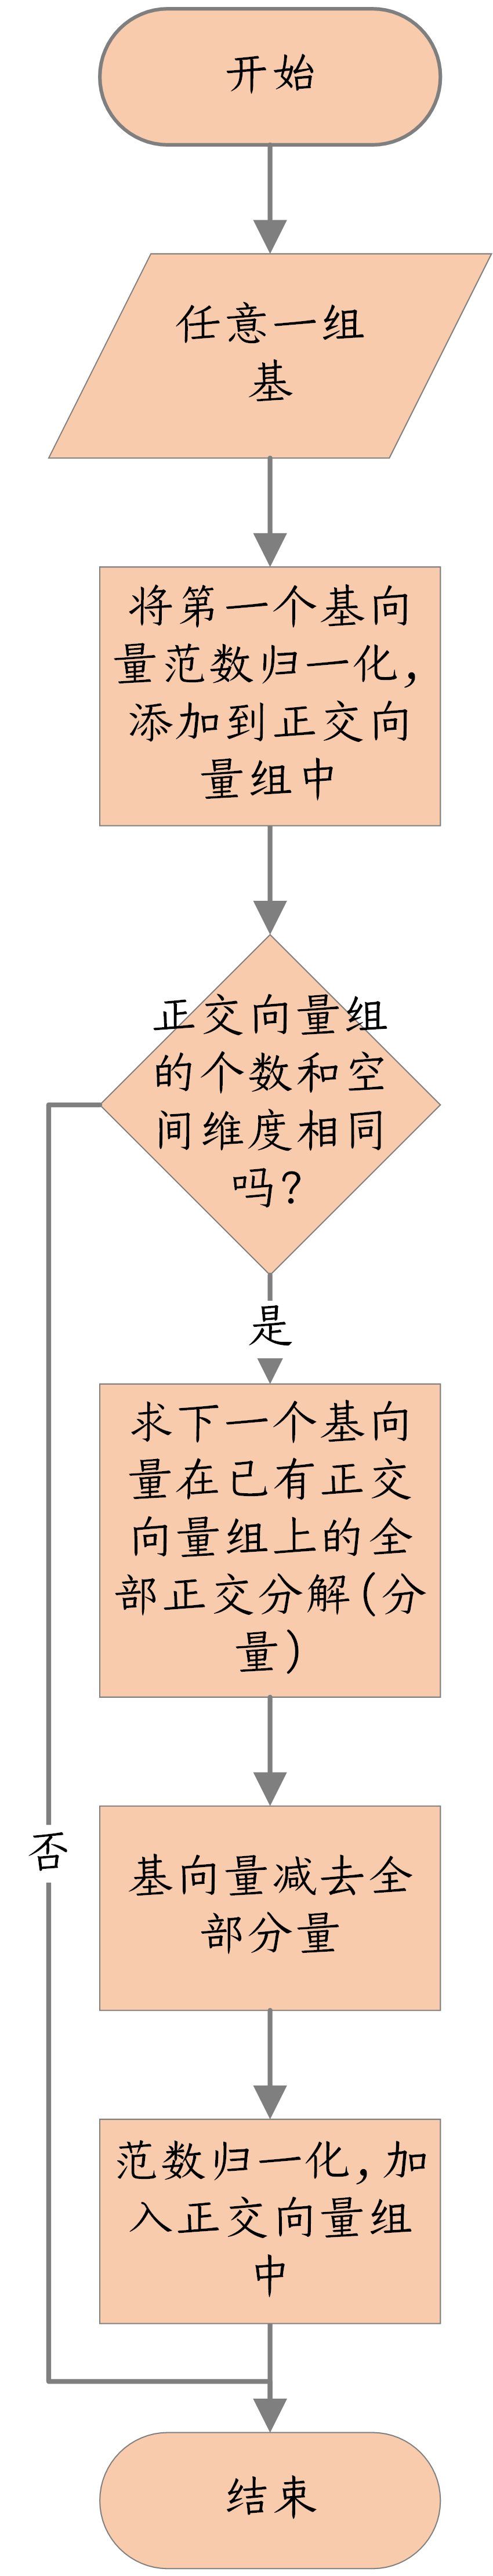
\includegraphics{Gram-Schmidt-procedure.png}
    \caption{Gram-Schmidt正交化程序}
\end{marginfigure}
\par Gram-Schmidt正交化程序直接给出了寻找标准正交基的方法(当然,这意味着\textcolor{BrickRed}{任何有限维内积空间都存在标准正交基})。
\par 我们上一章有结论——任意复指数空间的任意线性变换,都可以选取一组基使其矩阵为上三角形矩阵。我还想让这组基是标准正交的,我全都要,可以吗?彳亍。
\par \textcolor{BrickRed}{Schur's定理:任意复指数空间的任意线性变换,都可以选取一组标准正交基使其矩阵为上三角形矩阵;若线性空间的底域为\(\mathbb{R}\),该定理能否成立取决于上三角形矩阵的存在性。}\sidenote[][1cm]{直接对上三角矩阵这组基进行Gram-Schmidt正交化即可,上三角的等价条件并不会被破坏。}
\section{内积空间的线性泛函}
\par 显然,固定一个向量,内积运算就是一个线性泛函。逆天,其逆命题居然是成立的。\par \textcolor{BrickRed}{Riesz表示定理:任何有限维线性空间的任何线性泛函都可以表示成内积的形式。}
\[\forall \varphi \in \mathcal{L}(V,\mathbb{F})\;!\exists u\in V\; \forall v\in V\;(\varphi(v) = \langle v,u\rangle)\]
\[u = \overline{\varphi(e_1)}e_1 + \cdots + \overline{\varphi(e_n)}e_n\]
\section{正交补与最优化问题}
\par 给定一个子集\(U\),与全部元素正交的集合是其正交补\(U^\perp\)。\sidenote{\(U\)未必是子空间}
\[U^\perp := \{v\in V : \forall u \in U\; \langle v,u\rangle = 0 \}\]
正交补的基本性质
\begin{itemize}
    \item 正交补是子空间;
    \item \(\{0\}^\perp = V\;\wedge\;V^\perp = \{0\}\)
    \item \(U \cap U^\perp \subset \{0\}\)
    \item \(U \cap W \Rightarrow  W^\perp \cap U^\perp\)
\end{itemize}
\par 正交补提供了一种直和分解的自然方法。
\[U\text{ is a subspace of }V \Rightarrow V = U \oplus U^\perp\]
\newpage
可以推出
\[\dim U^\perp = \dim V -\dim U\]
\[U=(U^\perp)^\perp\]

\chapter{内积空间上的线性变换}
\section{自伴和正规变换}
伴随映射\sidenote{这是一种隐式定义,用Riesz表示定理理解——固定\(w\),泛函为\(\varphi(v)=\langle Tv,w\rangle\),然后\(u:=T^\ast w\)}
\[T:V\mapsto W,\;T^\ast := \langle Tv,w\rangle = \langle v, T^\ast\rangle \]
基本性质
\begin{itemize}
    \item 伴随映射是线性映射\(T^\ast \in \mathcal{L}(W,V)\)
\end{itemize}
% \begin{margintable}
%     \centering
%     \begin{tabular}{cc}
%         \toprule
%         命名 & 内容 \\
%         \midrule
%         \bottomrule
%     \end{tabular}
% \end{margintable}
\backmatter
% % \bibliography{}
% % \bibliographystyle{plainnat}
\printindex

\end{document}